\documentclass[12pt, a4paper]{article}
% Packages: 
\usepackage[utf8]{inputenc}
\usepackage[T1]{fontenc}
\usepackage[polish]{babel}
\usepackage[utf8]{inputenc}
\usepackage{lmodern}
\usepackage{graphicx}
\usepackage{indentfirst}
\usepackage{fancyhdr}
%------------------------------------
% Style config etc.:
\selectlanguage{polish}
\brokenpenalty=1000
\clubpenalty=1000
\widowpenalty=1000
\pagestyle{fancy}
\fancyhead{}
\fancyfoot{}
\rfoot{\thepage}
\lfoot{}
\lhead{}
\rhead{}
\renewcommand{\headrulewidth}{1pt}
\renewcommand{\footrulewidth}{1pt}
%--------------------
\title{Konfiguracja serwera DNS (Bind9) w systemie Linux Debian 11.}
\author{Marian Dorosz}
\date{}

\begin{document}

\maketitle
\newpage

\tableofcontents
\newpage

\listoffigures
\newpage

\section{Instalacja Bind9}
    \subsection{Pakiet instalacyjny}
        Instalacja aplikacji Bind9 na serwerze wymaga skorzystania z polecenia \textbf{apt-get install bind9}. Polecenie to zainstaluje aplikację w systemie. Po zakończeniu procesu instalacji można przystąpić bezpośrednio do konfiguracji.

\section{Generowanie klucza TSIG}

    \subsection{Czym jest TSIG?}
        TSIG (transaction signature) to protokół umożliwiający aktualizację bazy danych DNS w bezpieczny sposób. Najczęściej wykorzystuje się go do aktualizacji dynamicznego DNS, bądź serwerów DNS działających w trybie \textit{slave}. TSIG wykorzystuje klucze typu \textbf{shared secret}(w dużym skrócie chodzi o to, że komputery, które biorą udział w komunikacji znają klucz shared secret) w celu szyfrowania (w jedną stronę) wymiany informacji. Należy tutaj rozróżnić, że aktualizacja serwerów DNS (ich konfiguracji) różni się od wysłania zapytania do serwera (tzw. \textit{DNS query}).
        
    \subsection{Generowanie klucza TSIG.}
        Aby wygenerować klucz można skorzystać z polecenia \textbf{tsig-keygen} \\(można także użyć \textbf{dnssec-keygen}). 
        Wygenerowany klucz najlepiej zapisać w nowym pliku, który będzie dołączany do konfiguracji aplikacji bind9.
        \begin{figure}[!h]
            \centering
            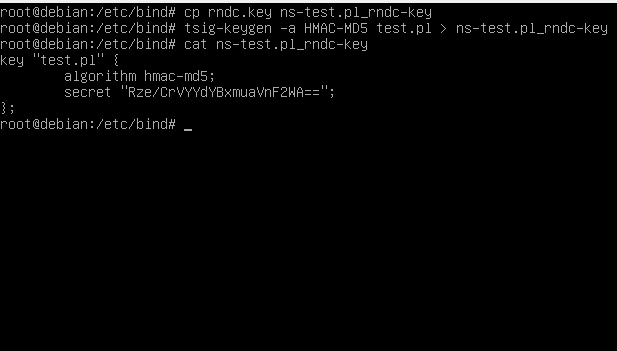
\includegraphics[width=\textwidth]{klucz_tsig.PNG}
            \caption{Generowanie klucza TSIG}
            \label{fig:TSIG}
        \end{figure}
        
\newpage
\section{Konfiguracja serwera DNS, rekordów RR oraz stref}

    \subsection{Konfiguracja pliku named.conf}
        Plik \textit{named.conf} jest głównym plikiem konfiguracyjnym serwera DNS.
        \begin{figure}[!h]
            \centering
            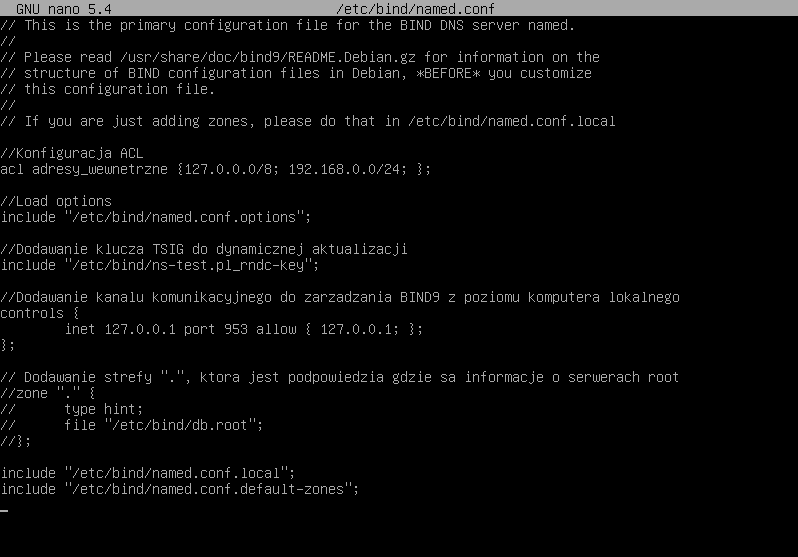
\includegraphics[width=\textwidth]{named_conf.PNG}
            \caption{Gotowy plik named.conf}
            \label{fig:named}
        \end{figure}
        
        \subsubsection{Konfiguracja ACL poleceniem: acl nazwa\_acl}
            ACL to lista adresów IP, które będą mogły podłączyć się do serwera DNS i go konfigurować.
            
        \subsubsection{Dodawanie klucza TSIG do dynamicznej aktualizacji}
            Jest to załączenie pliku z kluczem TSIG przy pomocy dyrektywy \textbf{include}.
            
        \subsubsection{Dodawanie kanału komunikacyjnego do zarządzania BIND9 z poziomu komputera lokalnego z wykorzystaniem RNDC (controls \{ ... \})}
            Zezwolenie na połączenie się z serwerem DNS przy pomocy RNDC z komputera o adresie 127.0.0.1 przy użyciu portu 953.

    \subsection{Konfiguracja pliku named.conf.options}
    
        Plik \textit{named.conf.options} zawiera wszystkie opcje konfiguracyjne dla serwera DNS.
        \begin{figure}[h!]
            \centering
            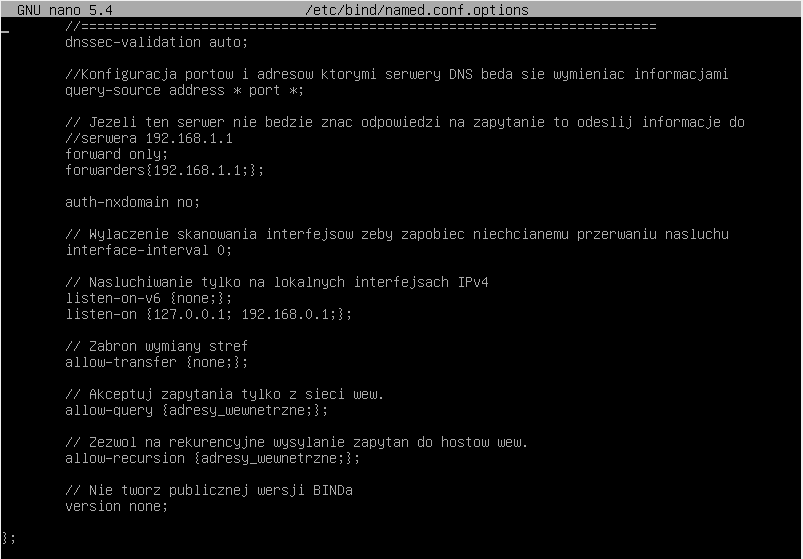
\includegraphics[width=\textwidth]{named_conf_options.PNG}
            \caption{Skonfigurowany plik named.conf.options}
            \label{fig:conf_opt}
        \end{figure}
        
        \subsubsection{Konfiguracja portów i adresów, którymi serwery DNS będą się wymieniać informacjami}
            Jak widać na powyższym obrazku poleceniem \textbf{query-source address * port *} zezwalamy serwerowi DNS na komunikację z serwerami o dowolnych adresach na dowolnych portach.
            
        \subsubsection{Konfiguracja serwera, do którego mają być przesyłane nierozwiązane zapytania}
            Opcje \textbf{forward only;} oraz \textbf{forwarders\{...\}} są informacją dla serwera, gdzie przesłać nierozwiązane zapytanie.
            
        \subsubsection{Nasłuchiwanie tylko na lokalnych interfejsach}
            Korzystając z poleceń \textbf{listen-on-v6: none; } oraz \textbf{listen-on \{...\}} powoduje, że serwer DNS nie będzie odpowiadał na zapytania pochodzące z adresów IPv6 oraz na zapytania przychodzące na adres inny niż wymieniony w nawiasach klamrowych.
        \subsubsection{Zablokowanie wymiany stref}
            Poleceniem \textbf{allow-transfer \{ none \}}; powoduje, że serwer nie będzie udostępniać informacji o strefach innym serwerom.
            
        \subsubsection{allow-query \{adresy\_wewnetrzne;\};}
            Polecenie to powoduje, że zapytania do serwera DNS będą mogły pochodzić z podsieci 127.0.0.1/8 (localhost) oraz 192.168.0.0/24. Wynika to z konfiguracji pliku z obrazu \ref{fig:named}.
            
        \subsubsection{allow-recursion}
            Pozwala na wysyłanie przez serwer zapytań do hostów pochodzących z dodanych ACL.

    \subsection{Konfiguracja pliku named.conf.local}
        W tym pliku konfiguruje się lokalne strefy DNS. W ustawieniach strefy należy dodać informację o typie strefy, o serwerach działających jako \textit{forwarderzy} oraz o bazach danych DNS i plikach z kluczami, które pozwalają na aktualizację wcześniej wspomnianych baz.
        \begin{figure}[!h]
            \centering
            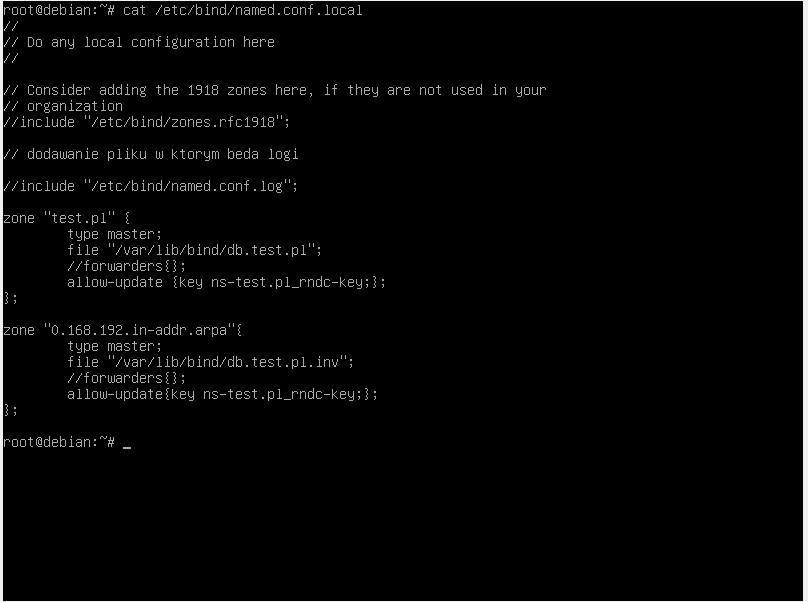
\includegraphics[width=\textwidth]{named_conf_local.PNG}
            \caption{Skonfigurowany plik named.conf.local}
            \label{fig:named_conf_local}
        \end{figure}
        
        \subsubsection{zone ''test.pl''}
            W ten sposób została dodana strefa test.pl. Jej typ to \textit{master}, a klucz, który zezwala na aktualizację tej strefy znajduje się w pliku \\ \textbf{''ns-test.pl\_rndc-key'';}. Plik z rekordami RR tej strefy ustawiony paramterem \textbf{file} to \\ \textbf{"/var/lib/bind/db.test.pl"}.
            
        \subsubsection{zone 0.168.192.in-addr.arpa}
            W ten sposób dodaje się strefę ARPA (tzw. \textit{odwrotny DNS}). Tak jak wcześniej dodana strefa test.pl strefa ARPA jest typu master, jej plik z rekordami RR to \textbf{"/var/lib/bind/db.test.pl.inv";}. Nie posiada ona żadnych serwerów działających jako \textit{forwarderzy}. Klucz umożliwiający aktualizację strefy to plik \textbf{''ns-test.pl\_rndc-key'';}.

    \subsection{Konfiguracja rekordów \textit{Resource Records}}
        \begin{figure}[!h]
            \centering
            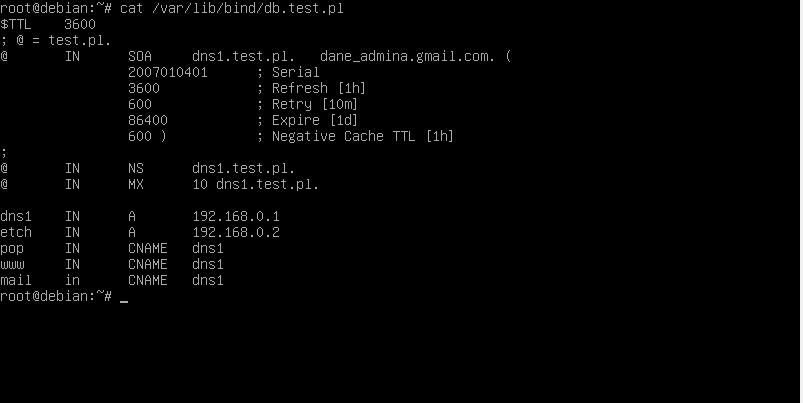
\includegraphics[width = \textwidth]{db_test_pl.PNG}
            \caption{Rekordy RR dla strefy test.pl}
            \label{fig:testpl}
        \end{figure}
        \newpage
        \begin{figure}[!h]
            \centering
            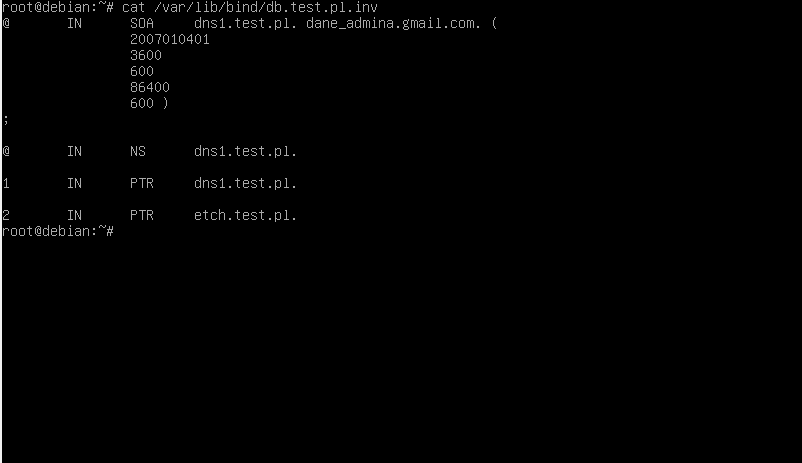
\includegraphics[width = \textwidth]{db_test_pl_inv.PNG}
            \caption{Rekordy RR dla strefy 0.168.192.in-addr.arpa}
            \label{fig:arpa}
        \end{figure}

        \subsubsection{Czym są rekordy RR?}
            Rekordy RR oznaczają jaki typ informacji przechowuje dana strefa DNS. Każdy rekord ma swój typ, czas, po którym wygasa oraz informacje specyficzne dla samego siebie.
            
        \subsubsection{SOA - Start of authority record}
            Rekord ten przechowuje autorytatywne informacje o strefie DNS, włączając w to główny serwer rozpoznawania nazw, email administratora, numer seryjny strefy oraz kilka liczników czasu, które powiązane są z odświeżaniem informacji o strefie. Liczniki te są informacjami dla serwerów zapasowych, które mają synchronizować się z głównym serwerem.
            
        \subsubsection{Rekord NS}
            Informacja dla serwera DNS o adresach pozostałych serwerów. Rekordy te mają wskazywać na rekordy typu A, które należy utworzyć w pliku.
            
        \subsubsection{Rekord A}
            Rekord używany do mapowania nazw, na adresy.
            
        \subsubsection{Rekord CNAME}
            Rekord ten jest rozszerzeniem rekordu A, czyli przekierowuje ``nazwę2 na nazwę1``, gdzie nazwa1 jest wcześniej nakierowana np. na adres 192.168.0.1.
            
        \subsubsection{Rekord MX}
            Rekord \textit{Mail Exchange} powstały na potrzeby usługi poczty elektronicznej. Przy pomocy tego rekordu oznacza się serwery poczty. Tak jak rekord NS, rekord MX musi być nakierowany na nazwę, która jest rozwiązana rekordem typu A.
            
        \subsubsection{Rekord PTR}
            Rekord mapujący adres IP na nazwę hosta. Używa się go w zapytaniach typu \textit{reverse DNS}
\newpage

    \subsection{Test przy pomocy narzędzia dig.}
        \begin{figure}[!h]
            \centering
            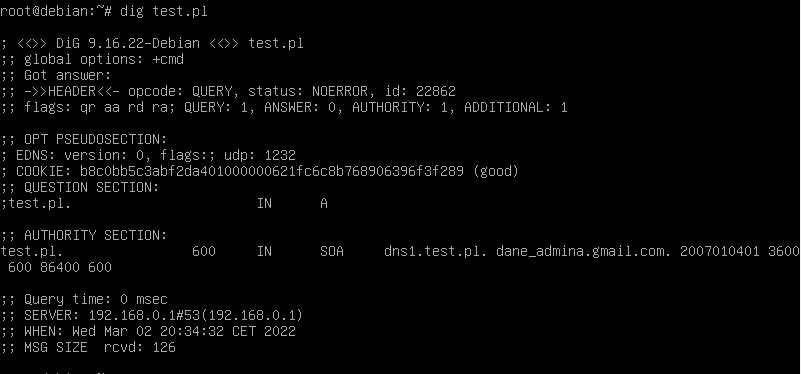
\includegraphics[width=\textwidth]{dig1.PNG}
            \caption{Wynik komendy Dig dla domenty test.pl}
            \label{fig:dig1}
        \end{figure}
        \begin{figure}[!h]
            \centering
            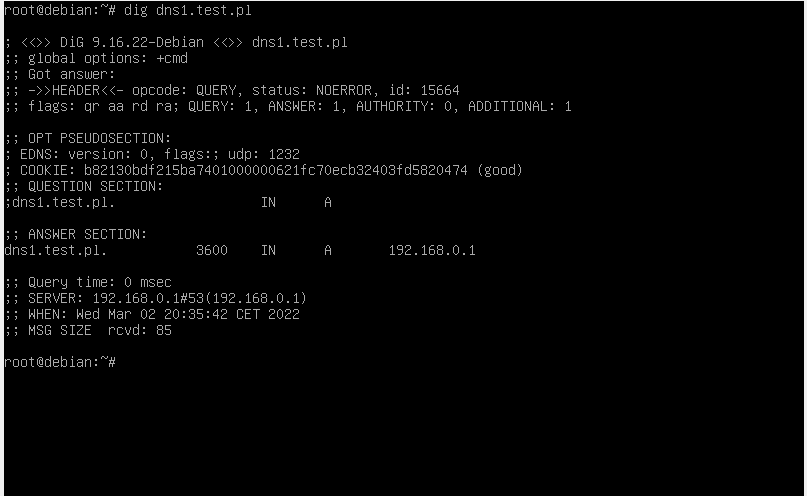
\includegraphics[width=\textwidth]{dig2.PNG}
            \caption{Wynik komendy Dig dla dns1.test.pl}
            \label{fig:dig2}
        \end{figure}
        Jak widać domena zwraca odpowiednie wartości rekordów, jeżeli zostanie ``wypytana`` przez narzędzie \textit{dig}. 

\end{document}
